\documentclass{article}

\usepackage[utf8]{inputenc}

\usepackage[
    backend=biber,
    natbib=true
]{biblatex}
\addbibresource{thesis.bib} %Import the bibliography file

\usepackage{hyperref}
\hypersetup{
    colorlinks=true,
}

\usepackage[pdf]{graphviz}
\usepackage{graphicx}
\usepackage{amsmath}
\usepackage{amsthm}
\usepackage{amssymb}
\usepackage{tikz}
\usepackage{freetikz}
\usetikzlibrary{shapes.geometric}
\usetikzlibrary{calc}
\usetikzlibrary{arrows, decorations.markings}
\usetikzlibrary{fit}
\usepackage{string-diagrams}
\usepackage{comment}
\usepackage{tabularx}
\usepackage[status=draft,layout=inline]{fixme}
\fxusetheme{color}
\usepackage{parskip}
\setlength{\parskip}{10pt} 
\usepackage{chngcntr}
\counterwithout{figure}{section}
\usepackage[normalem]{ulem}
\usepackage{listings}

\theoremstyle{definition}
\newtheorem*{ex}{Example}

\usepackage{etoolbox}
\newtoggle{plannthesis}
\toggletrue{plannthesis}
\newtoggle{incltitle}
\togglefalse{incltitle}

\title{E-graphs modulo theories (extended abstract)}
\author{Sofia Brookie}

\begin{document}

\maketitle

Note: accepted to EGRAPHS 2026 at PLDI

\section{Introduction}
E-graphs struggle with a combinatorial explosion when reasoning about certain theories. A notorious case is that of AC theories, those containing associative and commutative operators: the space complexity of equality saturation is doubly-exponential in the size of the input in the worst case.

Can equality saturation for AC theories be done in a more efficient way? There have been several proposals for extending E-graphs to \emph{E-graphs modulo theories} (\citep{zucker_omelets_2025_short}, \citep{panchekha_lin-graphs_2025}, \citep{shanabrook_custom_2026}). We want to combine \emph{theory-specific} reasoning methods for AC together with the general mechanisms of E-graphs and equality saturation in order to efficiently deal with AC theories. This approach is named after and inspired by the success of theory-specific methods in other automated reasoning tasks, such as in \emph{Satisfiability Modulo Theories} solvers (SMT solvers). The merits of a theory-specific approach in automated reasoning are advocated for in \citet{goos_little_2002_short}.

\subsection{An example}
The natural first step is to simply not add any different representations of terms that are equal up to AC; thus, nodes in the E-graph for AC operators will be variadic and we will consider their children unordered. This is the key idea from prior work (\citep{zucker_omelets_2025_short}, \citep{panchekha_lin-graphs_2025}, \citep{shanabrook_custom_2026}).

We will show that something extra is needed. Consider the equations
\begin{align}
	a + b &= b \\
	a + a &= c \\
	c + b &= d
\end{align}
taken modulo associativity of $+$.

We can represent them with an E-graph as follows:

\begin{figure}[h!]
	\centering
	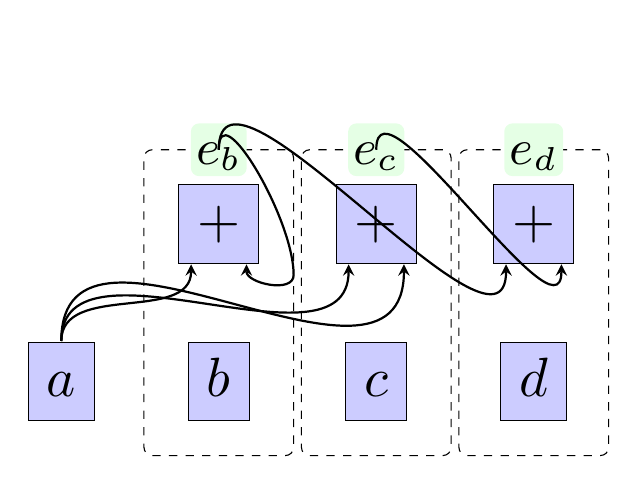
\begin{tikzpicture}[
			scale=2,
			transform shape,
			every node/.style={
					draw,
					fill=blue!20,
					text height=1.5ex, % Height above the baseline
					text depth=0.25ex  % Depth below the baseline
				}
		]
		\node (na) at (0, 0) {$a$};
		\node (nb) at (1, 0) {$b$};
		\node (nc) at (2, 0) {$c$};
		\node (nd) at (3, 0) {$d$};
		\node (nab) at (1, 1) {$+$};
		\node (naa) at (2, 1) {$+$};
		\node (nbc) at (3, 1) {$+$};

		\node[
			draw=none,
			fill=none,
			inner sep=12pt,         % Space between nodes and the box border
			fit=(nb) (nab),     % Tells TikZ which nodes to enclose
		] (box1) {};

		\draw[dashed, rounded corners=3pt]
		(box1.north east) --
		(box1.north west) node[midway, draw=none, fill=green!10, inner sep=1pt] {\small $e_b$} --
		(box1.south west) --
		(box1.south east) -- cycle;

		\node[
			draw=none,
			fill=none,
			inner sep=12pt,         % Space between nodes and the box border
			fit=(nc) (naa),     % Tells TikZ which nodes to enclose
		] (box2) {};

		\draw[dashed, rounded corners=3pt]
		(box2.north east) --
		(box2.north west) node[midway, draw=none, fill=green!10, inner sep=1pt] {\small $e_c$} --
		(box2.south west) --
		(box2.south east) -- cycle;
		
		\node[
			draw=none,
			fill=none,
			inner sep=12pt,         % Space between nodes and the box border
			fit=(nd) (nbc),     % Tells TikZ which nodes to enclose
		] (box3) {};

		\draw[dashed, rounded corners=3pt]
		(box3.north east) --
		(box3.north west) node[midway, draw=none, fill=green!10, inner sep=1pt] {\small $e_d$} --
		(box3.south west) --
		(box3.south east) -- cycle;
		
		\draw[->, >=stealth, thick] (na.north) to[out=90, in=270, looseness=1] ([xshift=-0.5em]nab.south);
		\draw[->, >=stealth, thick] (na.north) to[out=90, in=270, looseness=1] ([xshift=-0.5em]naa.south);
		\draw[->, >=stealth, thick] (na.north) to[out=90, in=270, looseness=1.2] ([xshift=0.5em]naa.south);
		\draw[->, >=stealth, thick] (box1.north) to[out=90, in=90, looseness=1]
		([yshift=0.5em]box1.east) to[out=270, in=270, looseness=1] ([xshift=0.5em]nab.south);
		\draw[->, >=stealth, thick] (box1.north) to[out=90, in=270, looseness=1] ([xshift=-0.5em]nbc.south);
		\draw[->, >=stealth, thick] (box2.north) to[out=90, in=270, looseness=1] ([xshift=0.5em]nbc.south);
		
	\end{tikzpicture}
\end{figure}

Consider the equation $b = d$, which follows from the simple deduction
\begin{align*}
	b = a + b = a + (a + b) = (a + a) + b = c + b = d
\end{align*}

However, $e_b$ and $e_d$ are two distinct E-classes in the E-graph! Why not?

The central step in the deduction relies on two different associations of the term $a + a + b$. The association $(a + a) + b$ is correctly assigned to class $e_d$, while the association $a + (a + b)$ is correctly assigned to the class $e_b$. However, given that we want to work modulo theories, we need to discover the fact that $e_b = e_d$, or we are throwing out some of the consequences derivable from the theory.

\subsection{How E-graphs handle ordinary critical pairs, but not AC-critical pairs}
To get a better perspective on this problem, we use ideas from rewriting and in particular the notion of Abstract Congruence Closure (\citep{bachmair_abstract_2000_short}). We can think of E-graphs as presenting a rewriting system, and the above E-graph as containing the rewrite rules

\begin{align*}
  b &\rightarrow e_b \\
  c &\rightarrow e_c \\
  d &\rightarrow e_d \\
	a + e_b &\rightarrow e_b \\
	a + a &\rightarrow e_c \\
	e_c + e_b &\rightarrow e_d
\end{align*}

(A distinguished equivalence class for $a$ is omitted to make the diagram easier to follow)

A critical pair for a rewriting system is a term that can be rewritten two different ways\footnote{It is also required to be minimal among such terms, but we gloss over this here}.
The perspective of Abstract Congruence Closure is that congruence closure, the core algorithm for `rebuilding' E-graphs, constructs a \emph{confluent term rewriting system} on an extended signature. Handling critical pairs is required for confluence, which ensures that a term rewrites into a single result; if we have a term $t$ that rewrites to both $e_a$ and $e_b$, we ought to automatically \emph{deduce} that the E-classes $e_a$ and $e_b$ should be merged.

By introducing new constants $e_1, e_2, \ldots$ as E-ids, we can `flatten' an input term $f(\ldots, g(h(\ldots)), \ldots)$ into just $f(\ldots, e_i, \ldots)$ and then assign it the name $e_k$ for some $k$. 

Now, to ensure the convergence of the rewrite system, we can look at two kinds of cases where a term could rewrite in two ways:

$e_1 \leftarrow f(\ldots e_i \ldots) \rightarrow e_2$ in which case, we ought to deduce that $e_1 = e_2$. This corresponds to merging E-classes which would contain duplicates of the same E-node.

$f(\ldots e_i \ldots) \rightarrow e_1$ and $e_i \rightarrow e_2$, in which case we ought to deduce that \\ $f(\ldots e_2 \ldots) = e_1$. This corresponds to canonizing the E-nodes using the union-find structure.

By fixpoint propagation, resolving these two cases are enough to resolve all cases of critical pairs with overlaps on more deeply nested subterms.

E-graph rebuilding can handle ordinary critical pairs, but this doesn't cover our above example, which is an \emph{AC-critical pair}. 

\subsection{Equality satuation: \\ handling AC-critical pairs by brute force}
E-graphs (not modulo theories) handle AC-critical pairs the same way as critical pairs for any other theory, with equality saturation: we \emph{ground} the AC identities by matching either side with the E-graph, and adding the equivalent other side (if it is not present) and merging the equivalence classes corresponding to either side.

Why do E-graphs fare poorly with AC? The two identities, (A) $\forall xyz.\; x + (y + z) = (x + y) + z$ and (C) $\forall xy.\; x + y = y + x$, can be semantically characterized as saying that two AC-terms are equal if they are equal as non-empty multisets of their subterms. Equality saturation will handle these identities by eventually deriving that an input term $a_1 + a_2 +  \ldots + a_n$, thought of as the multiset $\{a_1, a_2, \ldots, a_n\}$, is in the same E-class as every E-node of the form $s + t$ where $s$ and $t$ partition the multiset $\{a_1, a_2, \ldots, a_n\}$. There are $2^n - 1$ non-empty multisets $s$ and $t$ which we can partition a starting multiset of size $n$ into\footnote{If the multiset has an element of multiplicity more than 1, some of these will be the same, so this number will be reduced. However, we consider the worst case}, and one E-class will need to be generated for each. So, to reach saturation, we must create $O(2^n)$ E-classes, and it is easy to see that each E-class will, on average, have its own $O(2^n)$ E-nodes to represent every multiset partition of the multiset it represents.

These `redundant' E-nodes and E-classes play a role: any of the $O(2^{2^n})$ AC-subterms of the input could be part of an AC-critical pair, and so equality saturation eagerly assigns new E-classes to them, just in case. Introducing these extra E-classes and E-nodes is seemingly the best we can do in general unless we have a clever way to detect which ground instances of the identities are needed in order to ensure confluence modulo those identities.

In our above example, the associative identity would match against $a + (a + b)$, which is a term represented in our E-graph, and then merge this term (assigned to equivalence class $e_b$) with the corresponding other side of the associativity identity (assigned to equivalence class $e_d$  \emph{if} we have also added the instance of commutativity $c + b = b + c$ to the graph. Otherwise, adding this instance of commutativity later on and then rebuilding will correctly find the need to merge these classes).

\subsection{EMTs: Handling AC-critical pairs less na\"ively}
We don't need to add all AC-subterms to find critical pairs. It suffices to consider every pair of E-nodes with an AC symbol and check them for `overlap'. In our example, the E-nodes $a + e_b$ and $a + a$ form a potential critical pair $a + a + e_b$ as they overlap on the subterm $a$. We see that this implies the equation $a + e_b = e_c + e_b$, which can be added to the E-graph, which will merge the classes $e_b$ of the LHS and $e_d$ of the RHS.

This procedure always terminates (\citep{bachmair_abstract_2000_short}). It is, in fact, a special case of Buchberger's algorithm for finding Gr\"obner bases of sets of polynomials (\citep{tiwari_decision_2000_short}), a well-studied algorithm with a lot of work done in optimizing it to be fast enough in practice.

\section{Towards EMTs}
Seeing that resolving $T$-critical pairs is a key ingredient for E-graphs modulo $T$, we look to see if there are better ways to do this for certain $T$s (like AC) beyond the na\"ive, general approach of equality saturation.

We can show that this is equivalent to a known problem, the (uniform) word problem over $T$.

For AC, the word problem is known to be \textsc{Espace}-complete (\citep{mayr_complexity_1982_short}). This provides a theoretical lower bound on how much EMTs for AC can hope to achieve. Nonetheless, this is better than equality saturation for AC which takes doubly-exponential space, putting it in the class \textsc{EEspace}.

We can hope that AC will be solvable `fast enough in practice', as is typically the case for many problems such as SAT-solving. The connection with the well-studied Buchberger's algorithm makes this reasonable to hope for.

For A, the word problem is known to be undecidable (\citep{nyberg-brodda_g_2024_short}), so the best we can hope to achieve in general is provide an incremental method to find and resolve $T$-critical pairs, with no guarantee that this process will ever end. Nonetheless, working modulo A can improve on the expected cubic space overhead of the intermediate E-graphs created by equality saturation with A.

For certain theories, there are nicer bounds: Abelian groups, aka ACUN, have a word problem solvable in polynomial time by computing Hermite normal form. For vector spaces, even faster solving via Gaussian elimination is possible.

\subsection{Results}
We are currently implementing an EMT system that uses Buchberger's algorithm for AC. As we have argued, we need something like this to make an EMT system that 

\printbibliography

\end{document}